\chapter{System Identification}

System identification can be defined as the deduction of system characteristics from measured data. \cite{NASA-RP-1138} Process of system identification includes performing identification experiment to obtain data, determining an appropriate form of the model and estimating the unknown parameters of the model with some statistically based method. \cite{SoderstromStoica1989}

\section{Linear Regression}

Least squares approximation is probably the most common method of the linear regression and it can be used to to approximate the solution of overdetermined systems.

Parameters of line given by the following equation:

\begin{align}
  y = ax + b
\end{align}

\clearpage

best fitting to the data set of $n$ points is given as follows:

\begin{align}
  a &= \frac{\sum_{i=1}^{n}{ \left( x_i - \bar{x} \right) \left( y_i - \bar{y} \right) }}{\sum_{i=1}^{n}{ \left( x_i - \bar{x} \right)^2 }} \\
  b &= \bar y - a \bar x
\end{align}

Where:

\begin{align}
  \bar{x} &= \frac{\sum_{i=1}^{n}{ x_i }}{ n } \\
  \bar{y} &= \frac{\sum_{i=1}^{n}{ y_i }}{ n }
\end{align}

\begin{figure}[h!]
  \centering
  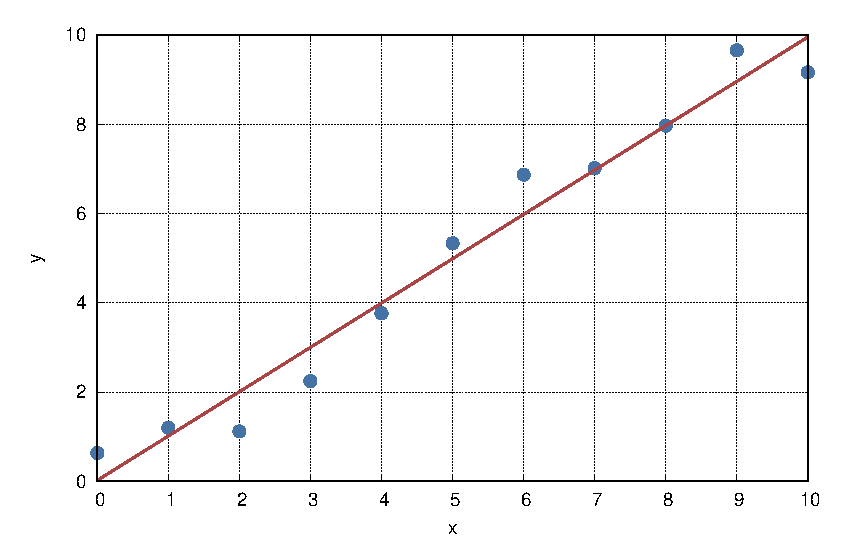
\includegraphics[width=140mm]{eps/linear_least_squares.eps}
  \caption{Linear Least Squares}
\end{figure}
